\documentclass{article}

\usepackage{graphicx}
\usepackage{tikz}

\newcommand{\shared}{This is a simple shared command.}
\providecommand{\ifpandoc}[2]{#2}


\graphicspath{{graphics}}

\begin{document}
  \begin{center}
    \shared

    \ifpandoc{We're using Pandoc !}{We're not using Pandoc !}

    
\includegraphics[height=5cm]{test.png}

    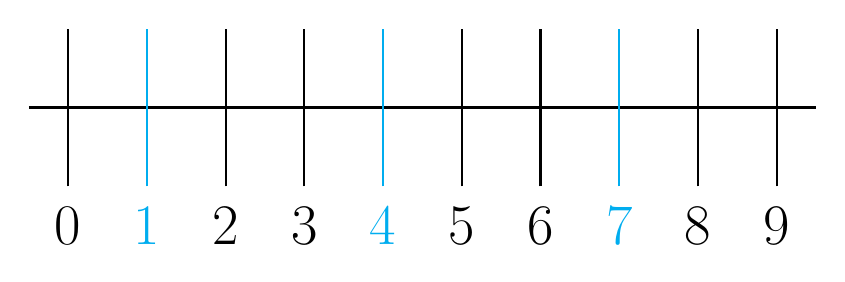
\begin{tikzpicture}
       \draw[thick] (-0.5,0) -- (9.5,0);
       \draw[thick] (0,-1) -- (0,1);
       \draw(0,-1.5) node {\fontsize{20}{30}\selectfont $0$};
       \draw[cyan, thick] (1,-1) -- (1,1);
       \draw(1,-1.5) node[text=cyan] {\fontsize{20}{30}\selectfont $1$};
       \draw[thick] (2,-1) -- (2,1);
       \draw(2,-1.5) node {\fontsize{20}{30}\selectfont $2$};
       \draw[thick] (3,-1) -- (3,1);
       \draw(3,-1.5) node {\fontsize{20}{30}\selectfont $3$};
       \draw[cyan, thick] (4,-1) -- (4,1);
       \draw(4,-1.5) node[text=cyan] {\fontsize{20}{30}\selectfont $4$};
       \draw[thick] (5,-1) -- (5,1);
       \draw(5,-1.5) node {\fontsize{20}{30}\selectfont $5$};
       \draw[thick] (6,-1) -- (6,1);
       \draw(6,-1.5) node {\fontsize{20}{30}\selectfont $6$};
       \draw[cyan, thick] (7,-1) -- (7,1);
       \draw(7,-1.5) node[text=cyan] {\fontsize{20}{30}\selectfont $7$};
       \draw[thick] (8,-1) -- (8,1);
       \draw(8,-1.5) node {\fontsize{20}{30}\selectfont $8$};
       \draw[thick] (9,-1) -- (9,1);
       \draw(9,-1.5) node {\fontsize{20}{30}\selectfont $9$};
    \end{tikzpicture}
  \end{center}
\end{document}
